\documentclass[dvipdfmx,a4paper]{ujarticle}

% パッケージ宣言
\usepackage{graphicx}

% ページレイアウト
\setlength{\hoffset}{-1in}
\setlength{\voffset}{-1in}
\setlength{\textheight}{297mm}
\setlength{\textwidth}{210mm}
\setlength{\topmargin}{0mm}
\setlength{\oddsidemargin}{0mm}
\setlength{\headheight}{0mm}
\setlength{\headsep}{0mm}

% ページスタイル
\pagestyle{empty}

% 本文
\begin{document}

% picture環境
\setlength\unitlength{1mm}
\begin{picture}(210,297)(0,0)

 % 背景（表示フォーマット）
\put(0,0){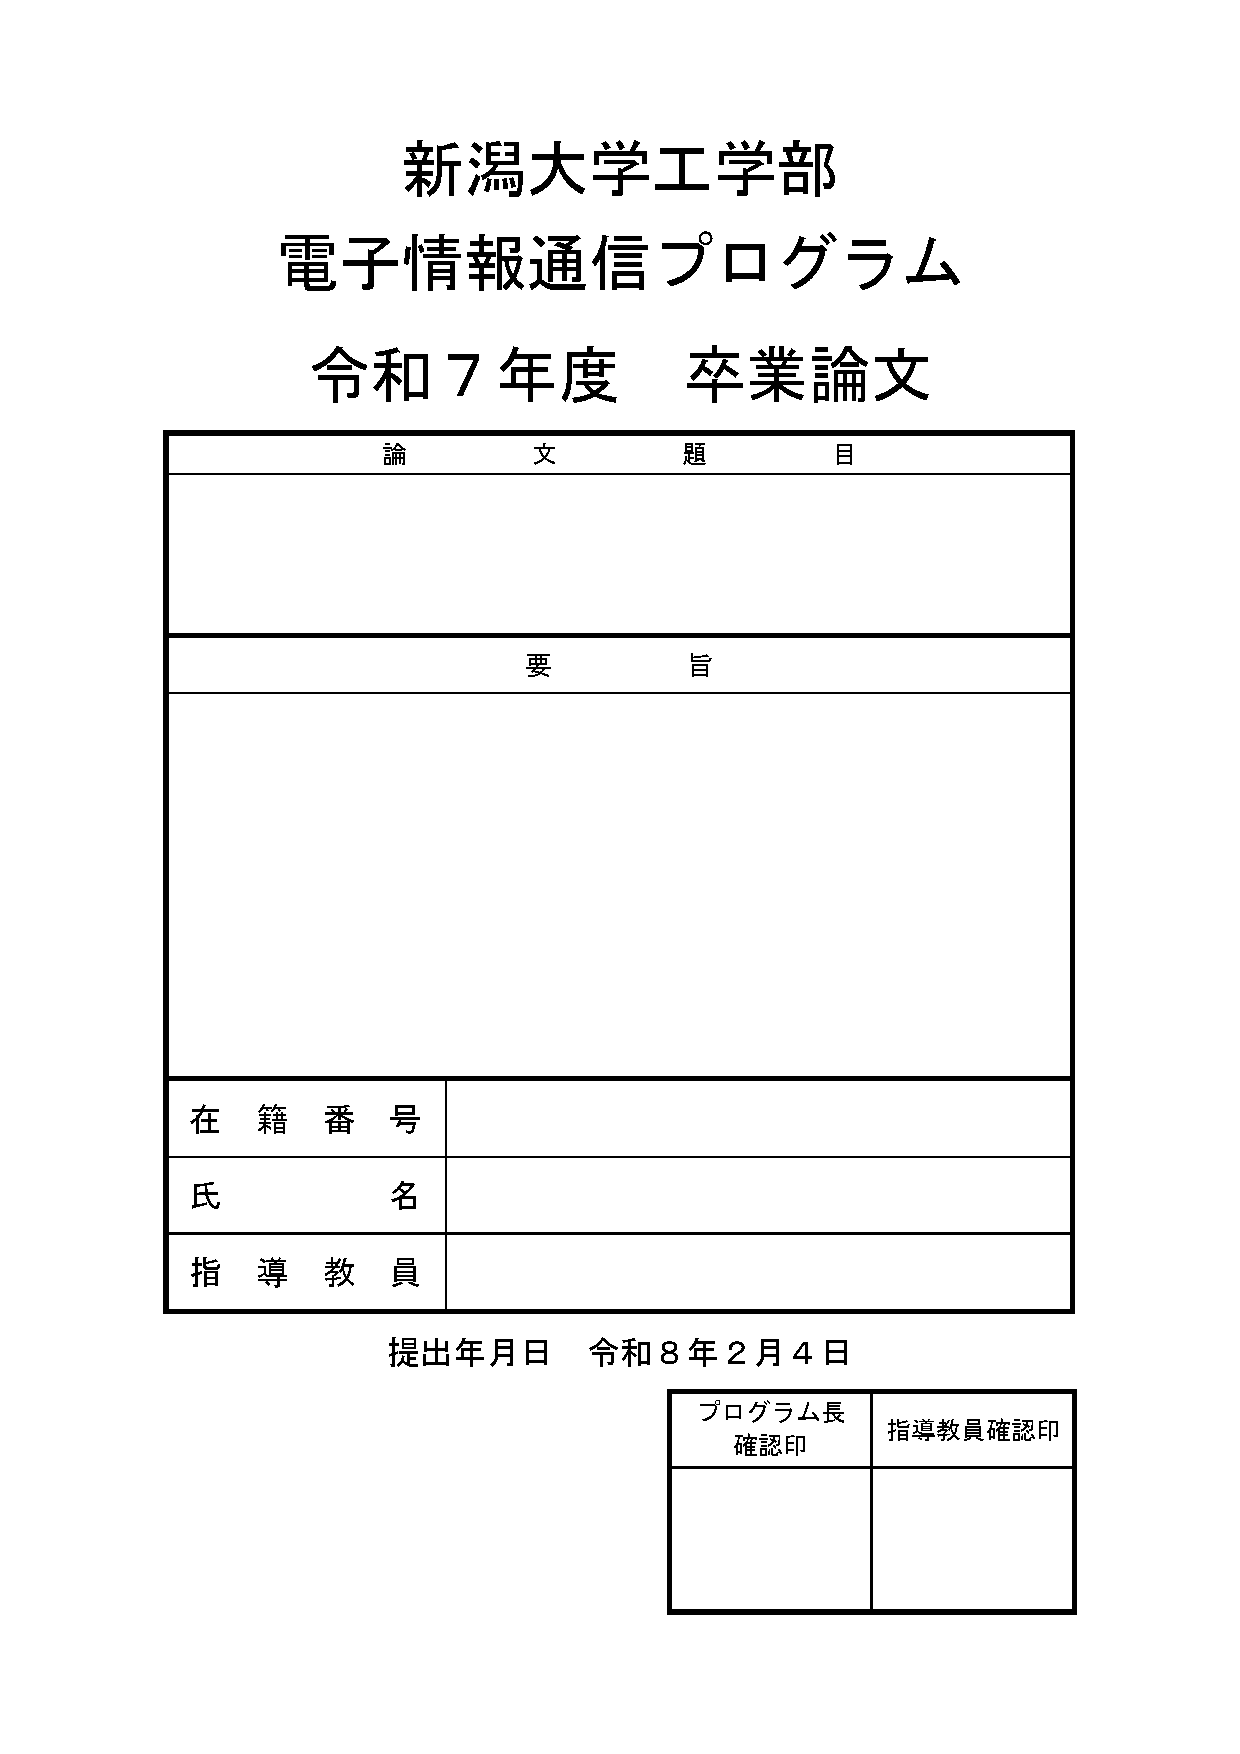
\includegraphics{sotsuron_hyoshi_bg.pdf}}
%\put(0,0){\includegraphics{kadaikenkyu_hyoshi_bg.pdf}}

 % 論文題目
 \put(32,202.2){\bf\fontsize{14}{16.8}\selectfont 
  \begin{minipage}[c]{145mm}\centering
  ○○のための○○のによる○○
  \end{minipage}
 }
 
 % 要旨
 \put(30,175.2){\fontsize{10.5}{18.0}\selectfont 
   \begin{minipage}[t]{149mm}
　本論文では，○○○○○○○○○○  のため，○○○○○○○○○○による○○○○○○○○○○を提案する(について検討する）．
   %
   ○○○○○○○○○○では，○○○○○○○○○○のため○○○○○○○○○○が求められている．
   ○○らは先行研究として○○○○○○○○○○した．○○○○○○○○○○により，○○○○○○○○○○を可能としている．
   %
   一方，○○○○○○○○○○は○○○○○○○○○○○○○○○○○○○○であり，○○○○○○○○○○○○○○○○○○○○の問題がある．
   %
    そこで本研究では，○○○○○○○○○○のために，○○○○○○○○○○○○○○○○○○○○を行う．
    %
    ○○○○○○○○○○○○○○○○○○○○を導入し，新たに○○○○○○○○○○○○○○○○○○○○を実現する．
   %
   ○○○○○○○○○○○○○○○○○○○○の実験を行い，○○○○○○○○○○を評価する．結果として，○○○○○○○○○○○○○○○○○○○○の有効性を確認する．   
   %
   \end{minipage}
 }
 
 % 在籍番号
 \put(78,106.2){\bf\fontsize{16}{19.2}\selectfont 
  \begin{minipage}[c]{100mm}\centering
  在籍番号
  \end{minipage}
 }

 % 氏名
 \put(78,93.2){\bf\fontsize{16}{19.2}\selectfont 
  \begin{minipage}[c]{100mm}\centering
  氏\quad 名
  \end{minipage}
 } 
 
 % 指導教員
 \put(78,80.2){\bf\fontsize{16}{19.2}\selectfont 
  \begin{minipage}[c]{100mm}\centering
  村\quad 松\quad 正\quad 吾\quad 教授
  \end{minipage}
 }  
\end{picture}
\end{document}